%% ---------------- From WR-ZEN article (EFTF2016) ------------------------
%
%The WR-ZEN is a new kind of WR node that incorporates
%a FPGA device and a hard ARM dual core microprocessor
%inside the same chip. The ARM is able to run a Linux kernel
%and this eliminates the need to use a conventional PC with an
%operating system. The flexibility of the platform has motivated
%that WR-ZEN is under study to be used in important scientific
%infrastructures such as Square Kilometer Array [11] (SKA)
%and Cherenkov Telescope Array [12] (CTA) among others.
%
%% ------------------------------------------------------------------------

The White Rabbit protocol requires a network topology similar to the ITU-T G.8275.1/Y.1369.1 standard, a IEEE-1588v2 telecommunication profile that describes a time-aware network capable to provide full timing support \cite{itu:TG8275_1_Y_1369_1} as explained in previous section. It uses a master time reference (SKA1 clock) that is distributed following a tree topology in a master-slave configuration. The SKA PPS distribution system is composed of two different kinds of devices: 

\begin{itemize}
	\item {The WR Switches \cite{sevensols:wr_switch}. They are standard 1U height rack-mounted equipment with 18 SFP ports and are placed in the CSPs at each of the clock ensembles. For SKA1-MID, one is placed halfway along each of the 3 spiral arms to regenerate the signal for the longest links.}
	\item{The end-nodes. They consist of a WR-ZEN node \cite{sevensols:wr_zen} powered by a Zynq FPGA-SoC and placed on inside a 1U rack enclosure. They will be located at the cores of SKA1-LOW and SKA1-SURVEY, along their spiral arms, one for each SKA1-MID dish and one for each CSP.}
\end{itemize}

The WR switches are responsible for generating the WR timing signal from the SAT clock ensembles. They lock to an external 10MHz reference and to a PPS signal, and use NTP or IRIG-B to determine the UTC time of each PPS edge. Synchronization between WR devices is performed over a a single fiber link up to 120 km using commercial SFPs.
However, the distances for SKA1-MID are longer and it is necessary to use 
intermediate WR switches as repeaters with a penalty over the system 
performance due to increment of the inherent noise of each WR device that it is 
propagated to the down-link nodes. An analysis of the jitter evolution for 
network with many hops could be read in \cite{torres2016scalability}. Thanks to 
network similarities between WR and SKA, both can use the same single fiber 
strand available for the SAT network. 

\begin{figure}[H]
	\centering
	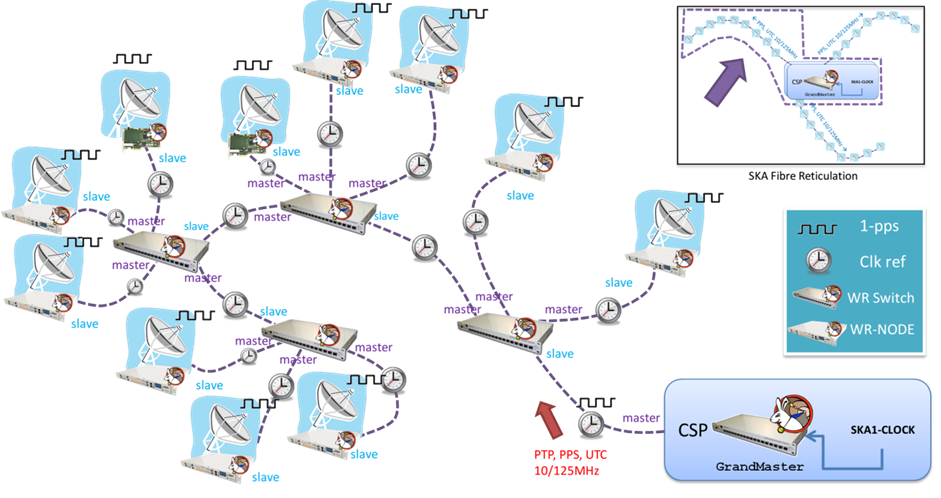
\includegraphics[scale=0.4]{img/ska_pps_network}
	\caption{Network topology for PPS signal distribution based on WR switches and nodes. The figure shows the different elements and the network topology. }
	\label{fig:ska_pps_dist_network}
\end{figure}

%\missingfigure{Example of a network topology for PPS signal distribution based on WR switches % and nodes}
 
An important feature of the system to take into account is that the PPS pulse itself at each station is derived from the reference frequency distributed from the SKA clock and not from the WR system. In normal operations, the WR system only monitors the absolute time of each PPS and reports it back activating an alert if the PPS signal does not align with the start of the UTC second. This condition indicates something is wrong in the timing chain and the station must be discard data to ensure not to introduce corrupt one in the system. Other functionality associated with the WR part is to temporarily alter the division ratio to bring the PPS edge back in alignment with UTC time. In this case, fringe finding must then be performed to restore full calibration again.

The centrally located WR switches and the WR end-nodes are connected to by a 
single strand of single-mode fiber with LC/PC connectors and industry standard 
bi-directional SFPs that use two wavelengths (down-link and up-link) to produce 
optical signals to be transmitted. Finally the end nodes generate a 1PPS signal available. 

As previously described, this solution requires WR switches and nodes. The 
former are well-defined equipment with known interfaces and software support. 
However, there is a problem related to the current WR nodes: they are based on 
PCIe interface cards to be plugged on standard computers, microTCA or VME-64 
crates and therefore, a specific computer is necessary to provide the high 
level software management functionalities. Although most of these cards can be used on 
stand-alone operation mode, they just use a FPGA device as processing engine 
and this make very complicated to add new functionalities or standard software 
tools. The main WR node designs include a soft-microprocessor on the FPGA gateware but it is not 
enough to fully solve the problem because it requires using complex 
non-standard firmware programming tools and it normally translates on high 
time-intensive development effort and makes difficult the upgrade of the system 
firmware.

As different solution, we have proposed the utilization of the ZEN board 
\cite{sevensols:wr_zen}. It is WR-compliant and powered by a Zynq FPGA-SoC device \cite{xilinx:zynq} that allows developing 
gateware and software on the same chip, tightly integrating performance and 
flexibility. Its new architecture is suitable to the utilization of 
software-hardware co-design strategies to take full advantages of the platform. 
Thus, the utilization of a host computer/crate to host the FPGA card can be avoided which reduces significantly the equipment price and is also a remarkable improvement in term of dependability which is a key factor taking into account that SKA Telescope should have an annual availability of about 95\% of the time (although degraded operation modes can be allowed under some circumstances).
Finally note that all these features are possible keeping the full flexibility of a complete CPU+FPGA system on a single board. 

In the following section we will describe the proposed node hardware, gateware and firmware that have been developed as a candidate solution for the SKA Telescope PPS distribution system. 

\subsection{A PPS distribution node architecture}

%% ------------------------ Javi ------------------------------------------
%% As a case of study, we can focus on the ZEN board that holds the Dual WRC (D-WRC), a revision from the original WRC developed by Seven Solution in our new line Xilinx 7 Series products. The D-WRC is %% able to synchronize two WR nodes or to be an intermediate link in a daisy chain network. In addition, the ZEN board includes high precision, low jitter and temperature compensated clock resources 
%% controlled by the D-WRC. Furthermore, the Dual core ARM Cortex processor, run under Linux OS, facilitating the development of user applications taking advance of the best from the WR technology and 
%% the ZEN resources. The on-board Linux allows the utilization of new and interesting features as webservices for configuration, SNMP support for status monitoring and remote firmware load and update. 
%% ------------------------------------------------------------------------

The PPS distribution system for SKA is based on the WR-ZEN platform that provides the WR support in order to ensure the synchronization accuracy in the system. The first design of the PPS system includes the Fine Delay FMC card that is used to generate the timing signals through mezzanine channels and has two Network Interface Cores (NIC) that allows accessing optical fiber ports as conventional Linux network interfaces.

Nowadays, the utilization of the Fine Delay FMC card is still under discussion and there is a possible design whose its final architecture could be addressed without this module.

\subsubsection{Hardware}
\label{subsec:hardware}

%% ---------------- From WR-ZEN article (EFTF2016) ------------------------
%
%The WR-ZEN is a small stand-alone board that integrates
%the latest Xilinx Zynq Z-7015 device with a Dual ARM
%Cortex-A9 MPCore with CoreSight and containing an Artix
%FPGA-logic with 74K logic cells, 380KB of embedded mem-
%ory and 160 DSP blocks. It has two optical SFP Ethernet
%interfaces, two copper Ethernet ports and the FMC expansion
%connector. On addition to FMC, a SAMTEC connector is
%available for developing of simple expansion boards and some
%USB sockets for monitoring. The WR-ZEN node is provided
%with improved oscillators, PLLs and a clocking scheme that
%provides significant better short term stability than previous
%WR node designs. It also includes several SMA outputs that
%can be configured to generate signals from the FPGA and an
%input that allows the WR-ZEN to behave as grandmaster. The
%WR-ZEN can be used with several FMC cards depending on
%the application: ADC, DAC, TDC, DDS, Fine delay, Digital
%I/O, etc.
%
%% ------------------------------------------------------------------------

%% ------------------------ Javi ------------------------------------------
%%The ZEN board is intended to be a high precise time provider and offers a large amount of possibilities facilitated by diverse connections and expansions:
%% - IRIG-B I/O: This is the Time of Day used by the ZEN board. It is able to work as master or slave.
%%- Two 10/100/1000 Ethernet ports connected to the ARM processors that can be used for diverse network applications and protocols (NTP, sNTP, PTPv2, management, etc..).
%% -Two SFP Cages where the WR compliant links are plugged.
%% -SMA connectors to enable the ZEN to synchronize itself with more precise clocks, e.g. GPS source or high stable oscillators, or providing a diverse set of clocks synchronized by WR.
%% - FMC connector to plug one of the mezzanine boards developed in the framework of the WR project or any other industrial one existing in the market. These FMC cards enhance the possibilities of the %%ZEN; e. g. FMC-ADC, FMC-DIO, FMC-FineDelay, FMC-DAC, etc; and allows many products configurations. 
%% - Memory resources; SD, DDR3, Flash.
%% - Two UART-USB connectors; for management and debugging in the D-WRC and Cortex processors.
%%In brief, the ZEN board offers to the final user a node capable to reach sub-nanosecond synchronization, working in daisy chain schemes, and provides the best of the Zynq and its new level of system %%design capabilities.
%% ------------------------------------------------------------------------

The WR-ZEN board is a proprietary design of the Seven 
Solutions company developed in 2015 aiming to improve the current designs of WR nodes.
The new platform includes a new family of SoC from Xilinx, the Zynq-7000. That family is characterized by joining a hard core microprocessor and a FPGA in the same chip. Hence, WR nodes, can achieve a performance increment while keeping costs low. The other key aspect of the new board design is the incorporation of a better clocking resources for the WR-logic and a more flexible clock schema that allows to generate a broad range of output synchronization signals very useful for custom designs which may need frequency sources different of 10 MHz.

\begin{figure}
	\centering
	\includegraphics[width=0.7\linewidth]{img/zenclkschema}
	\caption[WR-ZEN clocking schema]{The figure depicts the new clocking schema 
	presented in the WR-ZEN desing. The most relevant changes considering 
	previous designs are: the inclusion of an external PLL to lock an external 
	stable clock reference (GrandMaster mode), and a flexible path in the main 
	clocks path allowing the final user to choose between a low-noise PLL and a 
	full-featured PLL with many options such as programmable output delays.}
	\label{fig:zenclkschema}
\end{figure}

The Zynq-7000 SoC chosen is the XC7Z015. We will expose the 
key components under a WR point of view: the dual ARM Cortex-A9 MPCore allows the execution of a Linux based OS. There are enough computation resources to include other synchronization protocols, such as NTP or IRIG-B, full implementations of monitoring software, like SMTP, or to rise the WR PTP Core software logic from the LM32 to the ARM. A Dual-core architecture allows hybrid processing schemas, where a core is used by the Linux OS, and the other is focused on real time (RT) tasks such as the SoftPLL management. This could lead 
some research to avoid using the embedded LM32 soft-processor an ease the system development with all the code executed by the ARM processor. Xilinx calls that part \textit{Processing System}.

The Programmable Logic (PL) includes the FPGA resources needed 
by the design in Hardware Description Language, HDL, which includes the major part of the WR logic. For the XC7Z015, the PL part is equivalent to an Artix-7 FPGA. That concrete model includes 74000 logic cells, 380 KB of embedded memory and 4 Gigabit Transceiver Ports (GTP), more than enough for the WR implementation, allowing the inclusion of custom HDL modules for custom designs based on WR.

The board adds two Ethernet copper ports. In the current design, they are used mainly for remote management of the board, but in future developments, those ports would be connected to standard PTP devices via copper links. The WR-NIC drivers allow the communication and forwarding of packets between the copper Ethernet interfaces and the fibre ones used by the WR network. Other relevant connection included is the FMC HPC socket. In the current design the FMC Fine Delay board 
is supported but any of the FMC boards developed by the Open Hardware 
Repository (OHWR \cite{ohwr:repo}) community (among any other board using an FMC interface) could by added. For the SKA PPS distribution system, the Fine Delay FMC board \cite{ohwr:fmc-fine-delay} is used. It has four TTL output channels that can be programed to generate signals with different period and duty cycle properties. Moreover, it has a TTL input port and each of its four output channel can be set with an independent and variable delay in a range between 600ps and 120s respect to the input port. The Fine Delay FMC includes an ACAM TDC chip to implement all the functionalities described above. 

The WR-ZEN also includes a SAMTEC connector that is used to add extra circuitry to provide redundancy (duplicate power supply) and other additional components such as fans, LCD display, power supply control chips, etc.

The usual clock schema included in standard WR designs has been modified looking for an improvement of the clock stability and a more flexible schema to synthesize clock signals from the main clock reference used by WR. The new clock circuitry is depicted in diagram ??. The main WR crystal oscillator (XO) is replaced by a Crystek CVHD-950 with a nominal frequency of 50 MHz. This oscillator is better isolated and offers a lower noise profile compared to previous designs with the VM53S3 XO. Some phase noise plots are included in  \textit{ref a ??} showing a comparison between the new clock circuitry and the standard from previous WR designs. \klyonelnote{Aquí falta extender un poco esta parte, concretando las "bondades" del nuevo esquema de relojes. Creo que podemos simplemente describirlo sin tener que hacer un diagrama como habiamos planteado inicialmente.}

The main clock frequency is controlled by a Digital-to-Analog Converter (DAC) that receives the control values from the WR logic and tunes the oscillator's frequency to follow the clock reference from the master device in the network. The WR-ZEN's board adds a new DAC which offers better response time and stability compared to the previously used DACs. The main XO fed a PLL used to synthesize the required clock signals for the WR logic. Traditionally, WR designs used a PLL from Analog Devices, the AD9516-4. In this new design, a second PLL has been introduced between the main XO and the AD9516-4 PLL, the Texas Instrument LMK03806. The main reason is the better noise profile of this PLL that is used to latch the 10 MHz clock signal produced by the WR logic inside the PL. There is a jitter reduction of that signal due to the inclusion of the LMK, a phase noise comparison can be found in Fig. \ref{fig:zen_pn_all}. The AD9516-4 is maintained and receives the main clock source directly from the LMK thanks to an option of the later which allows to output the input clock signal without adding jitter. Designers can play with the clock schema in order to produce specific clock frequencies and they can choose which PLL is used to drive the GPTs or the WR logic.

\missingfigure{Figura del esquema de relojes de la ZEN}

% FIXME: Mira lo siguiente e integra lo que veas interesante...
%The WR-ZEN is a board designed by Seven Solutions company and contains a Xilinx Zynq SoC. %This SoC has a ARM dual core microprocessor (Cortex-A9 MPCore with CoreSight) and a FPGA %device (Artix with 74K logic cells, 380KB of embedded memory and 160 DSP blocks). This %versatile architecture removes the necessity of a conventional PC because all the high-level %software components can be implemented in the on-board processor. The WR-ZEN has been %conceived with an improved clocking scheme in relation to older WR nodes. It takes into %advantage of better oscillators and additional PLL to be capable to generate a wide range of %frequencies for several kind of different applications. The WR-ZEN is fully connected thanks %to its two optical fiber SFP interfaces and two RJ45 sockets and has other standard ports %such as FMC, SAMTEC, UART, I2C, SPI, etc. The expansion connectors (FMC and SAMTEC) are %though to add other boards that implement specific features or capabilities. Typical %applications for the FMC mezzanine board are Analog to Digital Converter (ADC), Digital to %Analog Converter (DAC), Time to Digital Converter (TDC), Fine Delay, Digital I/O (DIO), etc. %The SAMTEC connector is used to add extra circuitry to provide redundancy (duplicate power %supply) and other additional components such as fans, LCD display, power supply control %chips, etc.

\klyonelnote{Como dijimos y Javi apunta tenemos que poner otra foto más chula.}

\begin{figure}[H]
    \centering
    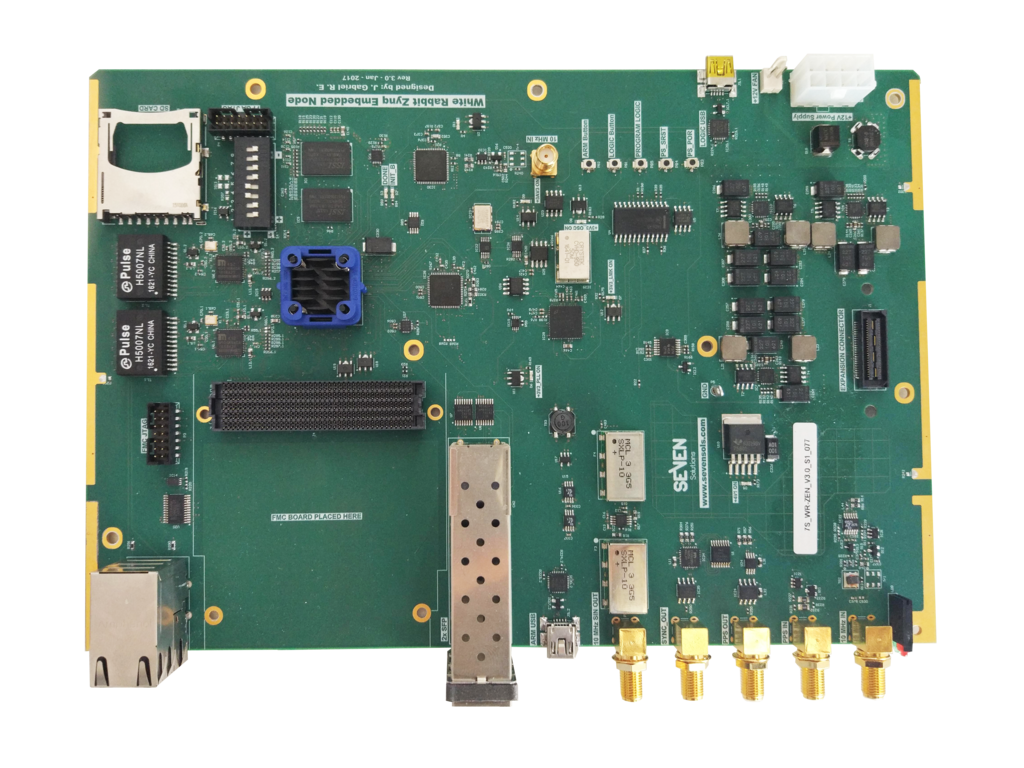
\includegraphics[width=0.7\linewidth]{img/wrzenv3_scaled}
    \caption[WR-ZEN board picture]{The picture shows the WR-ZEN board with the FMC Fine Delay connected. Main connectors are shown: Ethernet ports, SFP ports and the SMA connectors for the RF input/output signals.}
    \label{fig:wrzen}
\end{figure}


\subsubsection{Gateware}

%% ---------------- From WR-ZEN article (EFTF2016) ------------------------
%
%The gateware refers to the design that must be programmed
%in the Programmable Logic (PL) and the Processing system
%(PS) configuration to be applied. The PL is based on the Wish-
%bone (WB) bus [13] and has a main crossbar that interconnects
%the different IP cores.
%In the Fig. 2, the PL architecture is represented in more
%detail.
%* GIGABIT TRANSCEIVER PORTS (GTP): These
%blocks contain primitives to transfer data through a
%high performance dedicated interfaces. The GTPs are
%connected to the SFP sockets and allow to send/receive
%packets to/from the Gigabit Ethernet network.
%* WR PTP DUAL PORT CORE (WRPC-2P): It is the
%key core for WR nodes and contains all the elements
%needed to implement the WR protocol for two optical
%fiber ports.
%* AXI TO WB BRIDGE (AXI-WB BRIDGE): The PS
%must be able to talk to the PL. However, the PS
%uses the AMBA/AXI bus specification instead of the
%WB one of the PL. The AXI-WB bridge is able to
%convert from WB transactions to AXI transactions and
%viceversa.
%* FMC CORE: This IP core gives the specific function-
%alities for a certain kind of FMC card. In the reference
%design, the Fine Delay FMC core is included.
%* NETWORK INTERFACE CORE (NIC): It provides a
%network controller that is directly accesible from the
%Linux kernel. The NIC module can be managed like a
%standard network interface thanks to a specific driver.
%The gateware design carries out a WR compliant node
%with network capabilities and support for several FMC cards.
%However, the reference design only uses the Fine Delay FMC
%card, it can be extended easily to work with other cards such
%as DIO, TDC, ADC, etc.
%
%% ------------------------------------------------------------------------

The design gateware (FPGA firmware) is built on two different levels. The former uses the AMBA bus specification and considers the main elements for the Zynq ecosystem with several components such as Zynq Processing subsystem that takes care of configuring the ARM microprocessor and controlling the bus interconnections with it, a reset and clocking module that manages the clock and reset signals, an AXI QSPI core to program the hardware PLL chip, an AXI crossbar to glue everything together and a specific IP core that represents the next level of the design that is explained in following lines.

The design (shown in the Fig. \ref{fig:gateware_first_level}) is based on AXI and WB buses and has several crossbar modules to interconnect
all the components. Due to the different buses, there is an AXI-WB bridge that is responsible 
for converting AXI transactions into WB ones. This is necessary because the Zynq Processing System 
uses the AXI protocol but most WR compliant modules are based on Open Core WB bus. The WR Dual Port 
core implements the WR functionalities for the WR node. The main components of the WR Dual port core 
are the LM32 soft-microprocessor that runs a specific firmware with WR functions stored in the WB RAM, 
a WR endpoint that is charge of network transmissions/receptions over a 1 Gigabit Ethernet link, 
the WB PPSgen core that contains the timebase counter for the WR technology and the SoftPLL
that controls the servo loop algorithm to follow the master clock. The GT transceiver is a Xilinx primitive
that allows to implement high speed interfaces such as 1 Gigabit Ethernet links. The NIC cores are responsible
for receiving/sending packets between the ARM microprocessor and the network. The TxTSU module is a conventional
FIFO designed to store the transmission timestamps of the sent packets in order to give some time to the driver to
access them. The Fine Delay FMC core is a controller for the Fine Delay FMC mezzanine card. The main task for this 
board is to configure a delay to transmit a signal from the TTL trigger buffer to one of its four outputs.

%\missingfigure{Add figure to show first level architecture.}

\begin{figure}[H]
	\centering
	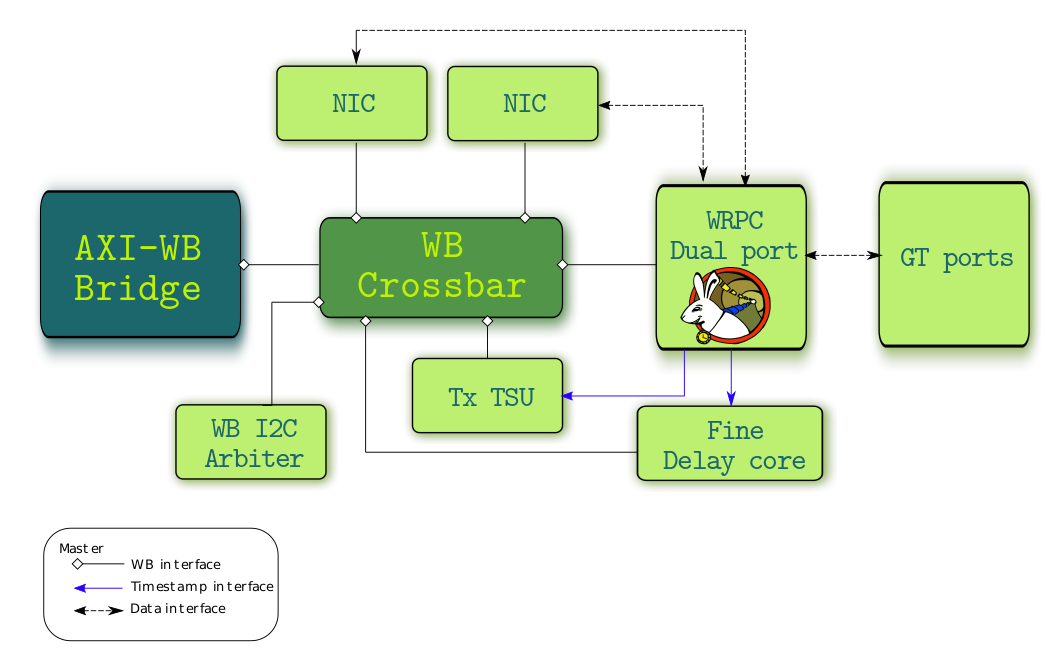
\includegraphics[scale=0.4]{img/gateware_first_level}
	\caption{Gateware project design. The figure shows the main components of the design. The most important one is the WRPC dual port that is responsible for implementing the WR protocol. The Gigabit Transceiver ports allows to transmit/receive packets to/from the network through the optical SFP modules. The NIC cores manage Ethernet packets and behave as standard network interface cards for the ARM microprocessor. The AXI-WB Bridge translates AXI transactions into WB ones. It is important because the ARM is connected using AMBA specification meanwhile the WR FPGA cores use Wishbone bus standard. Finally, the Fine Delay core contains the resources needed to control the Fine Delay FMC card.}
	\label{fig:gateware_first_level}
\end{figure}

The second level is referred to the specific IP core that takes into 
consideration the WR protocol and other basic features such as Gigabit 
networking, serial debug communication, timestamp mechanism, etc. This module 
uses the Wishbone Open Cores bus specification and is mainly 
vendor-independent. It is composed of many IP cores that are interconnected 
through a WB crossbar that allows bidirectional communication between any two 
IP cores. Moreover, the crossbar can store Self Descriptor Bus (SDB) 
information about the different components attached to it in order to discover 
them with a scan operation. Thanks to it, the WB peripherals can be discovered 
automatically by software tools and this allows not to hard-code the different 
addresses inside the source code improving the maintainability of the system. 

\subsubsection{Firmware}

The firmware code is related to all the functionalities needed by the White 
Rabbit protocol. In the node architecture, the embedded software part of the WR 
protocol and some device drivers runs in the soft-microprocessor describe in 
the previous section. The main tasks of the WR routines are the servo 
loop algorithm which, maintains the lock to the recovered frequency from the 
master device, and the implementation of the WR-PTP stack. In addition, a 
simple Command Language Interface (CLI) is introduced to allow 
the user interaction (think that some WR nodes can work in standalone mode and 
does not have an on-board hard microprocessor).

\subsubsection{Software}

%% ---------------- From WR-ZEN article (EFTF2016) ------------------------
%
%In this section, the software components needed to run a
%Linux kernel/Baremetal application on the WR-ZEN board are
%described. The Zynq devices needs a binary file (BOOT.bin)
%that is composed of a specific Xilinx bootloader known as First
%Stage Bootloader (FSBL), a gateware bitstream to program
%the FPGA and a baremetal application or a Second Stage
%Bootloader (SSBL) if Linux kernel must be loaded. The FSBL
%is encharged to initialize different peripherals, configure the
%FPGA with a bitstream and run the baremetal application
%or the SSBL. The baremetal application is encouraged to be
%coded with the Xilinx SDK because all the gateware details
%are imported to the software project and we can use all the
%functionalities of the Xilinx Board Package Support (BSP). On
%the other hand, the SSBL is a independent project and must be
%downloaded and compiled separately. The most common SSBL
%are U-boot [14] and Barebox [15]. The chosen bootloader is U-
%boot instead of Barebox because there is a Xilinx repository
%[16] that includes custom code for the Zynq devices. When
%everything is generated, the Xilinx SDK or bootgen tool must
%be used to pack all the binaries in a single file, the BOOT.bin.
%The following step is to compile the Linux kernel, kernel
%modules, libraries and userspace tools. To face this task, there
%are two ways. The first one is to compile every component
%separately and manually. It is very slow, tedious and error
%prone but it is the best way to control the different steps
%and customize them if necessary. On the other hand, there
%are some tools that automate the process such as Yocto [17]
%or Buildroot [18]. However, they present a disadvantage: the
%user loses the control and it is more difficult to add some mod-
%ifications because the tool does everything automatically. For
%the reference design, the Buildroot is used to ease and speed
%up the compilation of the Linux kernel, U-boot bootloader, the
%kernel modules and userspace tools. The Buildroot package is
%retrived from the official project website. It is very configurable
%and includes the Kconfig support to enable/disable the different
%features similar to the Linux kernel. Although the Buildroot
%eases very much the compilation process, it has many options
%and may be confusing for a non-expert user. To solve this
%issue, a set of scripts have been implemented to perform all
%the actions needed and configuration files for the Busybox,
%Linux kernel and the Buildroot are provided. This scripts are
%based on others from the WR Switch Software project [19] of
%the OHWR repository.
%In addition of the Linux kernel and the bootloader, some
%kernel modules and userspace tools for the WR-ZEN board
%have been written. The main kernel driver is the WR-ZEN
%carrier, known as zen, and is responsible for reprogramming
%the FPGA device and reading the EEPROM information of
%the WR-ZEN board. This driver is based on the fmc-bus
%[20] (OHWR) and it also gives NIC capabilities to manage
%the optical fiber ports as standard network interfaces from
%the Linux kernel. Some userspace tools to read/write the
%FPGA register (zenmem), reprogram the FPGA bitstrean (zen-
%fwloader.sh), reprogram the soft-microprocessor program (zen-
%cl) and send commands to the soft-microprocessor (zen-vuart)
%are included too. The driver and all these tools are inspired by
%the SPEC Software project [21] of the OHWR repository. As
%we saw in the previous section, the reference design has also
%a Fine Delay core that must be controlled by a specific kernel
%driver. Actually, there are two drivers (zio [22] and fmc-fine-
%delay [23]) and some userspace tools in the OHWR for the
%Fine Delay FMC card in a SPEC card. Using these ones as
%starting point, some minor modifications have been made to
%incorporated them to the WR-ZEN reference design.
%
%% ------------------------------------------------------------------------

The WR-ZEN is the first WR node taking advantage of a Linux 
based operative system (OS). Due to the inclusion of a dual-core ARM 
microprocessor in the platform, the system design is not longer tied to 
low-level software design. New functionalities, such as communication 
protocols, management tools and so on, are quickly added because of the 
facilities of an OS: a hardware abstraction layer, and drivers which abstract 
the management of the underlaying logic. This middleware adds also more 
security controlling the access to the hardware.

The counterpart is an increment in the complexity of the system design. The new platform takes advantage of its hard dual core microprocessor to deploy a Linux system or a standalone application.

In the SKA system, the WR-ZEN is used with a Linux 
kernel to ease the implementation of the specific applications and providing 
conventional mechanisms to add more functionalities and update the entire 
system in a fast and ease way which is not included in the current WR node 
embedded design. In order to build all the software components, some custom 
scripts (inspired by WR Switch Software project ones from OHWR) are added to 
allow user intervention and provides standard configuration for Linux kernel, 
Busybox and root filesystem.  
Moreover the basic Linux components, some userspace tools and custom kernel 
drivers have been developed to manage the main modules in the WR-ZEN reference 
design. The FMC kernel driver (\textbf{fmc}) is retrived from OHWR repository and it has not
been modified. Its main purpose is to implement a generic support for FMC bus
in the Linux kernel. The main driver for the WR-ZEN platform is the \textbf{zen} one
and manages all the IP cores in the design, create standard Linux network interfaces and
reprogram the FPGA with the proper bitstream. The \textbf{zio} driver is 
retrieved from OHWR
repository and it has not been modified. It creates the ZIO bus that exports driver attributes
through the SysFS. The \textbf{fmc-fine-del} module implements the Fine Delay FMC functions and
it is based on the OHWR repository one but includes some modifications to work properly in the
WR-ZEN platform. The \textbf{zen-nic} driver is responsible to enable/disable the network 
interface methods of the \textbf{zen} module.

As previously seen, there are dependencies between the different kernel drivers and it establishes the installation order. The \textit{zen} one depends on \textit{fmc}. The \textit{fmc-fine-del} needs \textit{zen}, \textit{zio} and \textit{fmc}. The \textit{zen-nic} only uses the \textit{zen}.

In addition to device drivers, there are several custom userspace tools related with drivers previous explained. Those that use the \textit{zen} driver API are \textit{zenmem} that is responsible for accessing memory map of the WR-ZEN IP cores, \textit{zen-fwloader} that programs the FPGA with a given bitstream, \textit{zen-vuart} and \textit{zen-cl} that allows talking to the soft-microprocessor (see the gateware section) and loading other firmware respectively. On the other hand, the  \textit{fmc-fine-del} driver has associated tools such as \textit{fmc-fdelay-board-time} that is used to get the current time, \textit{fmc-fdelay-pulse} that generates pulses with certain characteristics (frequency, initial delay, duty cycle, etc), \textit{fmc-fdelay-input} that prints some information when an incoming signal raises the input connector of the mezzanine card, \textit{fmc-fdelay-list} that enumerates the Fine Delay FMC cards plugged in the system (only one for WR-ZEN but however more for conventional PCs), \textit{fmc-fdelay-status} that check the status of Fine Delay FMC core and \textit{fmc-fdelay-term} that configures the termination of each channel among others.

Apart from the Linux or standalone environment described before, more 
components are needed  for the WR-ZEN platform. Previously any application or 
Operating system can run, a specific bootloader must initialize some hardware 
devices. In the Zynq technology, there is a special bootloader known as First 
Stage Bootloader (FSBL) that is responsible for early initializations and it is 
the first step to perform in whatever system based on Zynq. The FSBL sets up 
different peripherals, configures the FPGA with a bitstream and runs the 
standalone application or the Second Stage Bootloader (SSBL) which finally 
loads the Linux kernel in the RAM memory and prepare the system to run the 
specific user applications.

\begin{figure}[H]
	\centering
	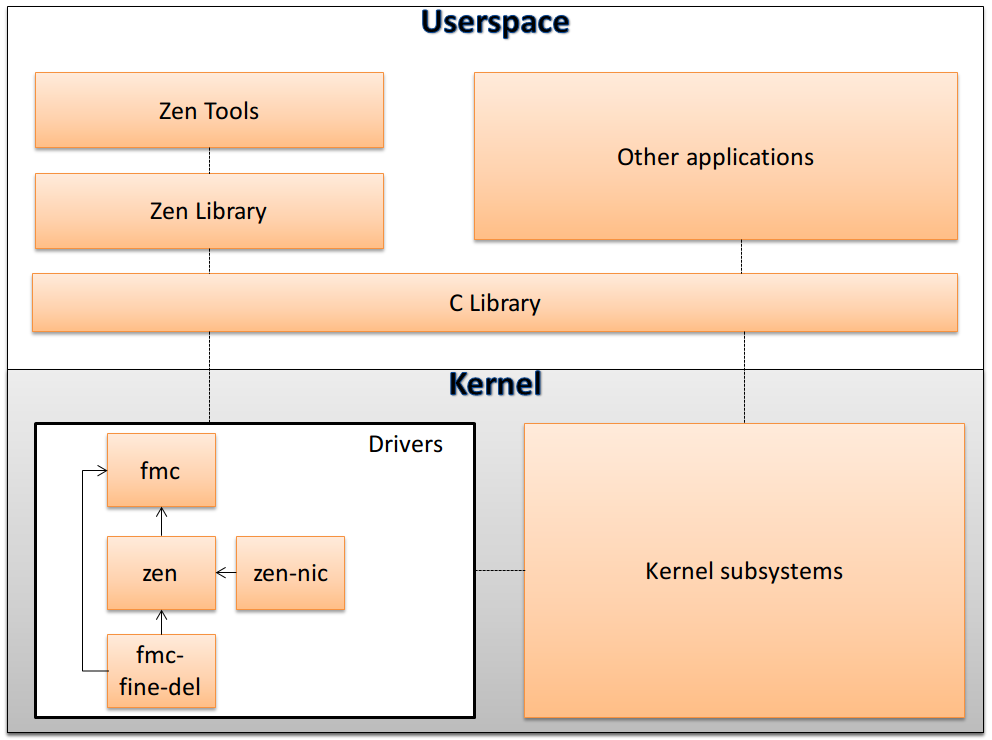
\includegraphics[scale=0.4]{img/software_architecture}
	\caption{Software architecture. The picture shows the software architecture
		used by the design. It is based on Linux kernel and several tools and drivers
		have been developed for the WR-ZEN board. The tools can be used to program 
		the FPGA, update the soft-microprocessor code or connect to the virtual UART
		interface of the WRPC-2p. They call the Zen Library procedures that finally
		use C Library functions and switch to kernel mode through system calls. In the
		kernel space, the drivers are responsible for implementing all the requested 
		functionalities. }
	\label{fig:software_architecture}
\end{figure}
